\documentclass[14pt]{extarticle}

\usepackage[utf8]{inputenc}
\usepackage[T2A]{fontenc}
\usepackage[russian]{babel}

\usepackage[a4paper,vmargin=20mm,lmargin=30mm,rmargin=15mm]{geometry}

\usepackage{amsmath,amssymb,amsfonts}
\usepackage{theorem}

\usepackage{amsmath}
\usepackage[normalem]{ulem}
\usepackage{enumitem}
\usepackage[linesnumbered,ruled,vlined,titlenotnumbered]{algorithm2e}

\usepackage{indentfirst}
\usepackage{graphicx}

\renewcommand{\topfraction}{1.0}
\renewcommand{\bottomfraction}{1.0}
\renewcommand{\textfraction}{0.0}

\graphicspath{{./images/2D/}}

\usepackage{listings}
\usepackage{lmodern}  % for bold teletype font
\usepackage{amsmath}  % for \hookrightarrow
\usepackage{xcolor}   % for \textcolor

\lstset{
  basicstyle=\ttfamily,
  columns=fullflexible,
  frame=single,
  breaklines=true,
  postbreak=\mbox{\textcolor{red}{$\hookrightarrow$}\space},
  rulecolor=\color{blue!80!black},
  language=[Sharp]C
}


\usepackage{setspace}
\onehalfspacing

% Перевод плагина algorithm2e

\SetKwInput{KwData}{Исходные параметры}
\SetKwInput{KwResult}{Результат}
\SetKwInput{KwIn}{Входные данные}
\SetKwInput{KwOut}{Выходные данные}
\SetKwIF{If}{ElseIf}{Else}{если}{тогда}{иначе если}{иначе}{конец условия}
\SetKwFor{While}{до тех пор, пока}{выполнять}{конец цикла}
\SetKw{KwTo}{от}
\SetKw{KwRet}{возвратить}
\SetKw{Return}{возвратить}
\SetKwBlock{Begin}{начало блока}{конец блока}
\SetKwSwitch{Switch}{Case}{Other}{Проверить значение}{и выполнить}{вариант}{в противном случае}{конец варианта}{конец проверки значений}
\SetKwFor{For}{цикл}{выполнять}{конец цикла}
\SetKwFor{ForEach}{для каждого}{выполнять}{конец цикла}
\SetKwRepeat{Repeat}{повторять}{до тех пор, пока}
\SetAlgorithmName{Листинг}{лислинг}{Список алгоритмов}


\theorembodyfont{\rmfamily}
\newtheorem{definition}{Определение}


\begin{document}
\begingroup
       \fontsize{12pt}{12pt}\selectfont

\begin{titlepage}
    \begin{center}
    МИНИСТЕРСТВО ОБРАЗОВАНИЯ И НАУКИ РОССИЙСКОЙ ФЕДЕРАЦИИ\\
    Федеральное государственное автономное образовательное учреждение\\
    высшего образования\\
    УРАЛЬСКИЙ ФЕДЕРАЛЬНЫЙ УНИВЕРСИТЕТ\\
    имени первого Президента России Б.\,Н.\,Ельцина\\
    \vspace{\baselineskip}
    ИНСТИТУТ ЕСТЕСТВЕННЫХ НАУК И МАТЕМАТИКИ\\
    \vskip +2cm
    Кафедра вычислительной математики и компьютерных наук\\
    \vspace{\baselineskip}
    \textbf{МНОГОМЕРНЫЙ АЛГОРИТМ ОВЫПУКЛЕНИЯ РОЯ ТОЧЕК, НАХОДЯЩИХСЯ В НЕОБЩЕМ ПОЛОЖЕНИИ}\\
    \vspace{\baselineskip}
    Направление \\09.04.03 «Прикладная информатика»\\
    \vskip +1cm
    \begin{tabular}{ l l }
    Допустить к защите: & Магистерская \\
    \hspace{3cm} & диссертация \\
    Зав. кафедрой: & \hspace{3cm}\\
     & \textbf{Корабельников}\\
    \hspace{3cm} & \textbf{Алексей Алексеевич}\\
    \hspace{3cm} & \hspace{3cm}\\
    \underline{\hspace{7cm}} & \underline{\hspace{7cm}}\\
    \hspace{3cm} & \hspace{3cm}\\
    Нормоконтролер: & Научный руководитель:\\
     & к.ф.-м.н. доц.  С. С. Кумков\\
    \hspace{3cm} & \hspace{3cm}\\
    \underline{\hspace{7cm}} & \underline{\hspace{7cm}}

    \end{tabular}

    \vfill

    Екатеринбург\\
    {2020}

    \end{center}
\end{titlepage}
\endgroup
\newpage
\setcounter{page}{1}
\thispagestyle{empty}

{
\setstretch{1.0}

\section*{\centerline{РЕФЕРАТ}}

% \noindent
% \bigskip
\noindent
Корабельников А. А. МНОГОМЕРНЫЙ АЛГОРИТМ ОВЫПУКЛЕНИЯ РОЯ ТОЧЕК, НАХОДЯЩИХСЯ В НЕОБЩЕМ ПОЛОЖЕНИИ, выпускная квалификационная работа: стр.~\pageref{lastpage}, рис.~???,
библ.~???~назв.

\medskip

{\raggedright

\noindent
Ключевые слова: ВЫПУКЛАЯ ОБОЛОЧКА, МНОГОМЕРНОЕ ЕВКЛИДОВО ПРОСТРАНСТВО, НЕОБЩЕЕ ПОЛОЖЕНИЕ ТОЧЕК.

}

\medskip

\noindent
Целью работы является разработка и реализация алгоритма построения выпуклой оболочки многомерного роя точек в случае их необщего положения. Под необщим положением точек подразумевается ситуация, когда в $(d-1)$-мерной гиперплоскости пространства $R^d$ измерения лежит больше, чем $d$ точек. Процедура реализует метод заворачивания подарка. Особенностью предлагаемой версии алгоритма является то, что после нахождения плоскости очередной гиперграни проводится построение выпуклой оболочки подроя точек, попавших в аффинное пространство этой гиперплоскости. Этот рекурсивный переход в пространство меньшей размерности проводится тогда, когда точек слишком много, чтобы образовать симплициальную гипергрань. В процессе построения гиперграни накапливается информация о её гиперрёбрах, необходимая для перехода к соседним граням. В целом, алгоритм заворачивания подарка реализует поиск в ширину в графе, в котором вершины соответствуют граням конструируемой выпуклой оболочки, а рёбра соединят вершины, соответствующие граням, имеющим общее гиперребро. Предложенный алгоритм реализован в виде программы на языке~C\#.

}

\newpage

\def\contentsname{\centerline{СОДЕРЖАНИЕ}}
\tableofcontents

\newpage
\section*{Введение}
\addcontentsline{toc}{section}{Введение}
Одной из важных проблем вычислительной геометрии является построение выпуклой оболочки конечного набора точек. При этом, очевидно, выпуклая оболочка является многогранником соответствующей размерности. На текущий момент существует множество алгоритмов, весьма эффективно решающих эту проблему на плоскости (см., например,~\cite{bib:preparata:eng,bib:preparata,bib:deBerg,bib:Ivanov}). Эти алгоритмы широко применяются для решения задач в геометрическом моделировании, распознавании образов, экономике, статистики, теории управления, дифференциальных играх и во многих других областях.

Однако переход в пространства более высокой размерности резко усложняет ситуации. Основная проблема при этом~--- необщее положение точек в овыпукляемом рое. Если в $(d-1)$-мерной гиперплоскости пространства $R^d$ лежит больше, чем $d$ точек обрабатываемого роя, то положение называют необщим.

При необщем положении точек роя может получиться так, что в гиперплоскости очередной гиперграни находится слишком много точек. Соответственно, требуется выяснение того, какие из этих точек являются вершинами выпуклой оболочки, а какие нет. Кроме того, важной информацией при работе алгоритмов овыпукления является соседство граней, которое выражается через информацию о гиперрёбрах, общих для тех или иных пар граней. Соответственно, в случае, когда грань не является симплексом соответствующего пространства, нахождение её гиперрёбер также требует дополнительных усилий.

В случае плоскости эти проблемы не возникают. В этом случае размерность гиперграни равна~1, грани являются отрезками, и несимплициальные грани возникнуть в принципе не могут. Если на грани~--- на отрезке~--- оказывается несколько точек, то очень легко выяснить, какие из них являются концами отрезка, а какие нет. Также многоугольник на плоскости имеет весьма эффективное представление в виде списка вершин, перечисленных в порядке обхода многоугольника по или против часовой стрелки. Эти обстоятельства и обеспечивают эффективность алгоритмов, производящих овыпукление на плоскости~\cite{bib:preparata:eng,bib:preparata,bib:deBerg}.

В трёхмерном пространстве ситуация несколько ухудшается, поскольку появляются описанные проблемы. Однако на помощь приходит естественная идея: после получения плоскости очередной грани, в которой лежит больше трёх точек, можно произвести овыпукление подроя точек, попавшего в эту плоскость. При этом используются алгоритмы для работы на плоскости, поэтому, в целом, процедура получается достаточно простой и по-прежнему эффективной~\cite{bib:Ivanov}.

Однако если и дальше увеличивать размерность, то гиперграни уже в свою очередь имеют размерность~3 или выше и не допускают удобную работу с ними.

Если наложить на овыпукляемый рой условие общности положения, это снимет указаненые проблемы: все гиперграни выпуклой оболочки гарантированно будут гиперсимплексами, не нужны будут никакие дополнительные вычисления для их получения и получения их гиперрёбер. Такие алгоритмы реализованы в современных популярных библиотеках алгоритмов вычислительной геометрии CGAL (бесплатная) и LEDA (платная). Библиотеки реализованы для языка C++. Но эти процедуры неприменимы в случае, когда в плоскости какой-либо гиперграни находится слишком много точек. В этом случае работа алгоритмов происходит некорректно, даже если грани реально являются гиперсимплексами.

Вследствие этого актуальной задачей является разработка эффективной процедуры построения выпуклой оболочки роя точек многомерного пространства, находящихся в необщем положении.

Традиционно для реализации алгоритмов, нацеленных на работу в многомерном пространстве, выбирается алгоритм Джарвиса, алгоритм заворачивания подарка, как наименее использующий специфику плоскости. Однако его нужно адаптировать для случая необщего положения точек, добавив определение ситации потенциально несимплициальной гиперграни и рекурсивный вызов в подпространстве меньшей размерности для обработки таких ситуаций. Кроме того, в случае наличия несимплициальных граней, которые в свою очередь могут иметь несимплициальные гиперрёбра и т.д., нужны нетривиальные структуры данных для хранения все информации об этих гипергранях и их соседстве.

В рамках выпускной квалификационной работы была поставлена цель разработать алгоритм построения выпуклой оболочки конечного набора точек в многомерном пространстве, находящихся в необщем положении, а также сопутствующие структуры данных для хранения результатов его работы. Также была запланирована программная реализация созданной процедуры.

\newpage
\section{Основная часть}

\subsection{Базовые определения и обозначения}

\begin{definition}[\cite{bib:kokichi}]
\emph{Выпуклой оболочкой} множества $P \subset R^d$ называется пересечение всех выпуклых подмножеств пространства~$R^d$, содержащих~$P$. Выпуклая оболочка множества $P$ будет обозначаться $CH(P)$ (от английского <<convex hull>>, <<выпуклая оболочка>>)
\end{definition}

Пусть $P = \{p_1, p_2, \ldots, p_n\} \subset R^d$, $d \geqslant 2$~--- конечное множество точек в $d$-мерном евклидовом пространстве. Несложно понять, что выпуклой оболочкой $CH(P)$ будет замкнутый многогранник в пространстве $R^d$ или, если $P$ вложено в какое-то аффинное подпространство, в этом подпространстве.

\begin{definition}
Из двух точек пространства $R^d$ точка $p_1$ считается меньше точки $p_2$ \emph{в лексикографическом порядке}, если найдется индекс $1 \leqslant i^* \leqslant d$ такой, что $p_{1,i^*} < p_{2,i^*}$ и для всех $1 \leqslant i < i^*$ имеем $p_{1,i} = p_{2,i}$. Здесь и далее символ $p_{k,i}$ означает $i$-ю координату точки $p_k$.
\end{definition}

Символом $\langle \cdot, \cdot \rangle$ будет обозначаться скалярное произведение в евклидовом пространстве~$R^d$. Символом $|\vec n|$ будет обозначаться длина вектора $\vec n$: $|\vec n| = \sqrt{\langle \vec n, \vec n\rangle}$.

Для ненулевого вектора $\vec n$ обозначим через $\vec n_0$ вектор, сонаправленный с $\vec n$ и имеющий единичную длину: $\vec n_0 = \vec n / |\vec n|$.


\subsection{Алгоритм Джавриса на плоскости}
\label{sec:ch2}

Пусть дано множество точек $P = \{p_1, p_2, \ldots, p_n\} \subset R^2$. Требуется указать точки роя~$P$, являющиеся вершинами многоугольника $CH(P)$.

Идея алгоритма Джарвиса (алгоритма заворачивания подарка) заключается в следующем:

1) находится какое-нибудь ребро многоугольника выпуклой оболочки и объявляется текущим;

2) с текущего ребра переходим к следующему, пока не будет достигнуто начальное ребро. После этого $CH(p)$ считается построенной.

\medskip

Для построения начального ребра проделываются следующие действия. Находится точка из роя $P$, минимальная в лексикографическом порядке. Пусть это точка $p_1$. Через неё проводится прямая, параллельная оси $Oy$. Иными словами, прямая, перпендикулярная оси~$Ox$. Затем эта прямая поворачивается вокруг точки $p_1$ против часовой стрелки, пока она коснется одной или нескольких других точек. Самая дальняя от $p_1$ точка из тех, которых коснулась прямая, назначается вторым концом начального ребра. Пусть это точка $p_2$.

\medskip

Пусть имеется текущее ребро с концами в точках $p_i$ и $p{i+1}$, причём точка $p_{i+1}$ была найдена после точки $p_i$. Тогда поворачиваем прямую $(p_ip_{i+1})$ вокруг точки $p_{i+1}$ против часовой стрелки, пока она не коснётся одной или нескольких других точек. Самая дальняя от $p_{i+1}$ точка из тех, которых коснулась прямая, назначается вторым концом нового ребра. Пусть это точка~$p_{i+2}$.

Если ребро $[p_{i+1}p_{i+2}]$~--- это начальное ребро $[p_1p_2]$, алгоритм заканчивает работу, а найденные точки $p_1$, $p_2$, \ldots, $p_i$ являются вершинами многоугольника выпуклой оболочки $CH(P)$, перечисленными против часовой стрелки.

\medskip

Видно, что центральным местом данного алгоритма является процедура поворота прямой вокруг заданной её точки до тех пора, пока она не коснётся других точек из набора. Формализуем эту процедуру.

Пусть вектор $l_i$~--- это единичный вектор, противоположно направленный вектору $\overrightarrow{p_ip_{i+1}}$ (то есть $l_i = (\overrightarrow{p_{i+1}p_i})_0$). Тогда нужные точки $\{p^i_1$, $p^i_2$, \ldots, $p^i_{k_i}\}$ роя $P$~--- это точки, на которых достигается минимум скалярного произведения $\langle l_i, (\overrightarrow{p_i, p_j})_0$, то есть такие точки, что угол между $l_i$ и $\overrightarrow{p_i, p_j}$ максимален среди всех точек роя.

При построении начального ребра считаем, что $l_0$~--- это орт положительного направления оси $Oy$.

\medskip

Тогда выбор первого ребра можно схематично представить шагами, изображёнными на рис.~\ref{fig:2D_1}--\ref{fig:2D_4}. Красная точка на рис.~\ref{fig:2D_1}~--- это $p_1$, лексикографически минимальная точка роя~$P$. На рис.~\ref{fig:2D_2} проведена прямая, параллельная оси $Oy$, и выбран вектор~$l_0$ (красная стрелка). yf hbc/~\ref{ig:2D_3} схематичнсо показан перебор точек роя в поисках второй вершины исходного ребра. Рис.~\ref{fig:2D_4} демонстрирует окончание этого процесса.

\begin{figure}[t]
  {}\hfill%
  \begin{minipage}{0.4\textwidth}
    \centering

    \hspace*{-0.1\textwidth}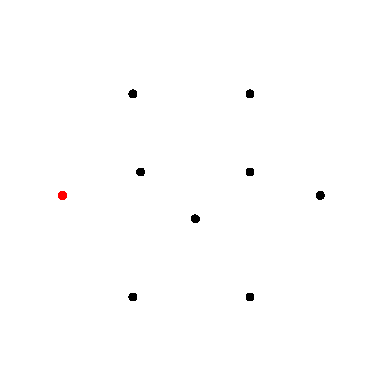
\includegraphics[width=1.25\textwidth]{gift1.pdf}

    \vspace*{-7ex}

    \caption{Поиск начального ребра: выбор лексикорграфически минимальной точки овыпукляемого роя; красным выделена точка $p_1$}
    \label{fig:2D_1}
  \end{minipage}
  \hfill
  \begin{minipage}{0.4\textwidth}
    \centering

    \hspace*{-0.1\textwidth}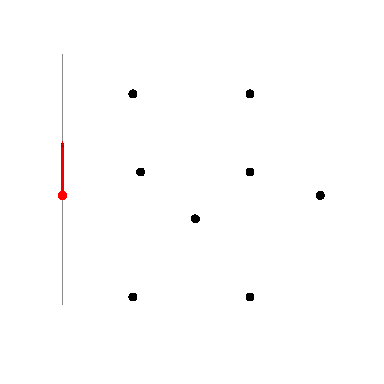
\includegraphics[width=1.25\textwidth]{gift2.pdf}

    \vspace*{-7ex}

    \caption{Поиск начального ребра: приближение к прямой начального ребра~--- вертикальная прямая}

    \label{fig:2D_2}
  \end{minipage}
  \hfill{}

  {}\hfill%
  \begin{minipage}{0.4\textwidth}
    \centering

    \hspace*{-0.1\textwidth}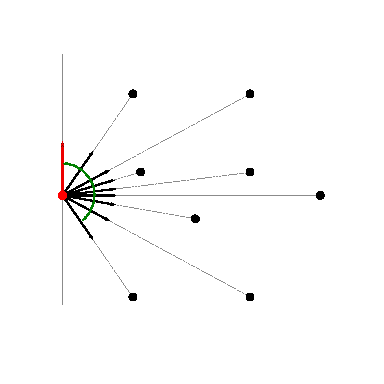
\includegraphics[width=1.25\textwidth]{gift3.pdf}

    \vspace*{-7ex}

    \caption{Поиск начального ребра: перебор точек в поисках тех, направление на которые от $p_1$ даёт максимальный угол с $l_0$}
    \label{fig:2D_3}
  \end{minipage}
  \hfill
  \begin{minipage}{0.4\textwidth}
    \centering

    \hspace*{-0.1\textwidth}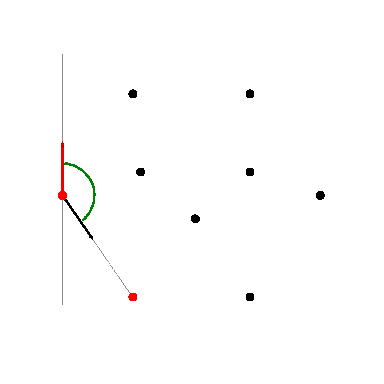
\includegraphics[width=1.25\textwidth]{gift4.pdf}

    \vspace*{-7ex}

    \caption{Поиск начального ребра: вторая красная точка~--- $p_2$, второй конец начального ребра~}
    \label{fig:2D_4}
  \end{minipage}
  \hfill{}
\end{figure}

Действия, направленные на поиск следующего ребра выпукло оболочки схематично показаны на рис.~\ref{fig:2D_5},~\ref{fig:2D_6}. На рис.~\ref{fig:2D_5} левая красная точка~--- это начало $p_i$ текущего ребра, правая красная точка~--- конец $p_{i+1}$ текущего ребра. Перебираются точки роя, в посках тех, направление на которые от точки $p_{i+1}$ даёт максимальный угол с вектором $l_i$ (красная стрелка). Рис.~\ref{fig:2D_6} показывает окончание этого процесса.

На рис.~\ref{fig:2D_7} показано окончание процесса построения выпуклой оболочки.

\medskip

Сложность данного алгоритма, очевидно, равна $O(hn)$, где $n$~--- количество точек в рое $P$, а $h$~--- количество рёбер выпуклой оболочки. Сложность вытекает из того, что при построении каждого из $h$ рёбер перебирается $n-1$ точка роя (кроме точки, вокруг которой поворачивает прямая текущего ребра).


\begin{figure}[t]
  {}\hfill%
  \begin{minipage}{0.4\textwidth}
    \centering

    \hspace*{-0.1\textwidth}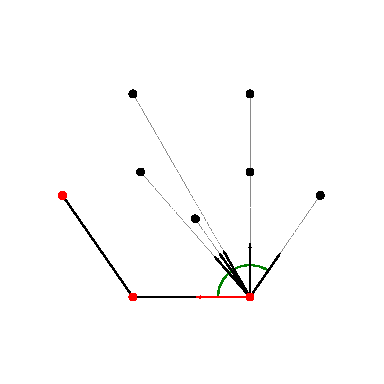
\includegraphics[width=1.25\textwidth]{gift8.pdf}

    \vspace*{-7ex}

    \caption{Поиск очередного ребра: перебор точек в поисках тех, направление на которые от $p_{i+1}$ даёт максимальный угол с $l_i$}
    \label{fig:2D_5}
  \end{minipage}
  \hfill
  \begin{minipage}{0.4\textwidth}
    \centering

    \hspace*{-0.1\textwidth}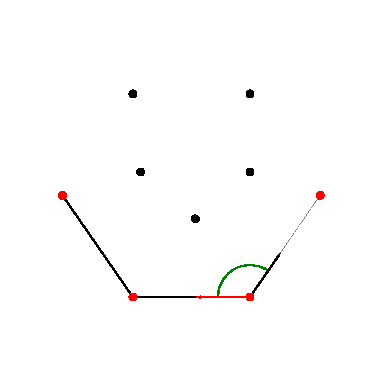
\includegraphics[width=1.25\textwidth]{gift9.pdf}

    \vspace*{-7ex}

    \caption{Поиск очередного ребра: выбор точки $p_{i+2}$, второй вершины очередного ребра}
    \label{fig:2D_6}
  \end{minipage}
  \hfill{}
\end{figure}

\begin{figure}[t]
  \centering

  {}\hfill
  \hspace*{-0.04\textwidth}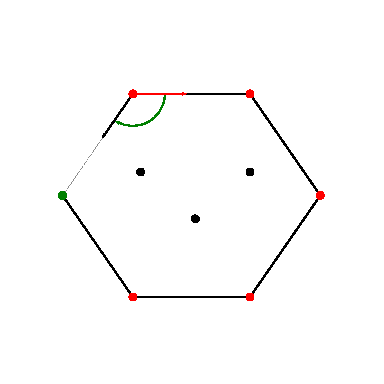
\includegraphics[width=0.5\textwidth]{gift13.pdf}
  \hfill
  \hspace*{-0.04\textwidth}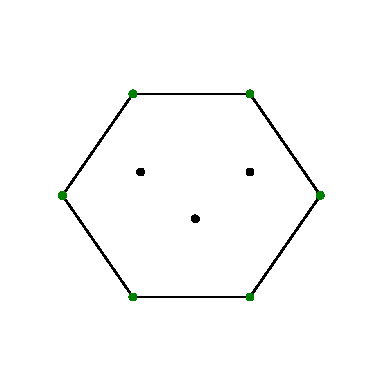
\includegraphics[width=0.5\textwidth]{gift14.pdf}
  \hfill{}

  \vspace*{-7ex}

  \caption{Окончание процесса построения выпуклой оболочки}
  \label{fig:2D_7}
\end{figure}

\subsubsection{Алгоритм заворачивания подарка в многомерном пространстве в случае общего положения точек}
\label{sec:gw3d}

В дальнейшем приставка \emph{гипер-} будет опускаться, когда из контекста будет понятно, об объекте какой размерности идёт речь. То есть под \emph{плоскостью} будет подразумеваться $(d-1)$-мерная гиперплоскость в пространстве~$R^d$, под \emph{гранью} $d$-мерного многогранника будет подразумеваться $(d-1)$-мерная гипергрань, а под \emph{ребром}~--- $(d-2)$-мерное гиперребро, или гипергрань (гипер)грани.

Пусть теперь базовое пространство, в котором находится рой $P$, имеет размерность $d > 2$. Кроме того, будем считать, что точки роя $P$ находятся в общем положении.

Вследствие этого предположения можно утверждать, что выпуклая оболочка $CH(P)$ есть многранник с гранями, какждая из которых есть $(d-1)$-мерный симлекс и задается $d$ точками. При этом других точек роя в плоскости грани нет.

Тогда в алгоритм Джарвиса произойдут следующие изменения.

На этапе построения начальной грани теперь надо совершить не один поворот исходной плоскости, перпендикулярной первой координатной оси, а $d-1$ поворот, чтобы плоскость <<легла>> на $d$ точек роя.

Формально процедура поворота плоскости вокруг ребра теперь выглядит следующим образом. Пусть имеется плоскость $\alpha$, задаваемая точками $p^\alpha_1$, $p^\alpha_2$, \ldots, $p^\alpha_d$. Пусть мы желаем повернуть её относительно ребра, задаваемого точками $p^\alpha_2$, \ldots, $p^\alpha_d$. Выполняются следующие действия:
%
\begin{enumerate}[topsep=-0.5\parsep,itemsep=-0.5\parsep]
  \item Строим ортонормированный базис ребра, вокруг которого происходит поворот. Для этого проводим процедуру ортонормирования Гра\-ма--Шмид\-та (см.,~например,~\cite{bib:Bekl}) набора из $d-2$ векторов $\overrightarrow{p_2p_3}$, $\overrightarrow{p_2p_4}$,~\ldots, $\overrightarrow{p_2p_d}$. Обозначим полученный ортонормированный набор векторов через $N = \{\vec n_i\}$, $i = 1$, \ldots, $d_2$.

  \item Построим вектор $\vec n'$, дополняющий набор $N$ до базиса плоскости $\alpha$. Для этого сделаем шаг процедуры Грама--Шмидта для вектора $\overrightarrow{p_2p_1}$ на фоне набора $N$. Заметим, что в силу сути действий, производимых при шаге этой процедуры, вектор $\vec n'$ будет направлен внутрь грани, задаваемой точками $p_k$.

  \item Перебираем точки роя $P$, за исключением точек $p^\alpha_1$, \ldots, $p^\alpha_d$. Для каждой взятой точки $p'_i$ строим вектор $\vec n_i$, дополняющий набор $N$ до базиса плоскости, определяемой точками $p'_i$, $p^\alpha_2$, \ldots, $p^\alpha_d$. Для этого делаем шаг процедуры Грама--Шмидта для вектора $\overrightarrow{p_2p}'_i$ на фоне набора $N$. Опять имеем, что полученный вектор $\vec n'_i$ направлен внутрь тетраэдра, задаваемого точками $p'_i$, $p^\alpha_2$, \ldots, $p^\alpha_d$.

  \item Перебирая точки $p'_i$, выбираем ту, для которой угол между векторами $\vec n'$ и $\vec n'_i$ наибольший, то есть для которых скалярное произведение $\langle \vec n', \vec n'_i \rangle$ наименьшее. В силу предположения об общем положении роя $P$ такая точка $p^*$ будет единственной.

  \item Точки $p^*$, $p^\alpha_2$, \ldots, $p^\alpha_d$ задают грань, имеющую общим ребро, задаваемое точками $p^\alpha_2$, \ldots, $p^\alpha_d$, с гранью, задаваемой точками $p^\alpha_1$, $p^\alpha_2$, \ldots, $p^\alpha_d$.
\end{enumerate}

\medskip

Заметим, что в случае построения начальной грани, плоскость, которую мы начинаем вращать, задаётся не набором точек. Действительно, мы проводим эту плоскость через точку $p_1$, лексикографически минимальную в наборе~$P$, перпендикулярно первой координатной оси. То есть эта плоскость задаётся одной точкой $p_1$ и своим базисом, который состоит координатных ортов $e_2$, $e_3$, \ldots, $e_d$.

В этом случае мы поочередно выкидываем первый вектор из этого набора, второй, третий и т.д., рассматривая оставшиеся как базис ребра, вокруг которого поворачиваем, а после нахождения новой плоскости, задаваемой точкой $p^*$, вставляем в набор вектор $\overrightarrow{p_1p}^*$ взамен исключенного. Соответственно, перед каждым очередным поворотом требуется провести ортонормирование имеющегося базиса ребра.

\medskip

Процедура перехода от начальной грани к соседним в отличие от случая на плоскости не имеет линейного характера, поскольку каждая грань уже имеет $d$ соседей (поскольку $(d-1)$-мерный симплекс, задаваемый $d$ точками, имеет $d$ рёбер, которые задаются каждым из $d$ наборов из $(d-1)$-й точки).

Для описания этой процедуры уместна графовая формализация.

Рассмотрим неориентированный граф, в котором вершины~--- это грани многогранника $CH(P)$. Две вершины $v_i$ и $v_j$ соединены ребром, если соответствующие им грани $\alpha_i$ и $\alpha_j$ имеют общее ребро. Наша задача~--- перебрать все вершины этого графа.

Этот перебор можно осуществить при помощи того или иного алгоритма поиска по графу. Однако при этом следует иметь в виду, что традиционно используемая рекурсивная реализация поиска в глубину, использующая системный стек, может быть чересчур накладной, так как многогранник $CH(P)$ может иметь достаточно большое количество граней. При <<ручной>> же организации сопутствующих структур данных более кдобным оказывается поиск в ширину. Именно он и был выбран для реализации.

При работе алгоритма поиска на графе важной структурой данных является структура, определяющая, была ли ранее посещена та или иная вершина. В случае, когда вершины графа~--- натуральные числа от 1 до максимального номера вершины, в качестве такой структуры выступает массив логических значений. Однако в рассматриваемой ситуации вершины графа имеют более сложную природу. Поэтому вместо массива разумно рассматривать хэш-словарь, хранящий логические выражения.

Такой подход, в свою очередь, приводит к необходимости определения разумной хэш-функции грани. Рассматривались следующие варианты вычисления хэша:
\begin{enumerate}[topsep=-0.5\parsep,itemsep=-0.5\parsep]
  \item упорядочиваем в лексикографическом порядке точки, определяющие грань, считаем их хэши и на основе полученного набора целых чисел считаем хэш грани;

  \item упорядочиваем индексы точек, определяющих грань, и на основе полученного набора целых чисел считаем хэш грани;

  \item уравнение плоскости, содержащей грань, и на основе коэффициентов уравнения строим хэш грани.
\end{enumerate}

Первые два способа хорошо работают в случае общего положения точек. Однако, если рой~$P$ не общего положения, то после получения плоскости очередной грани и отсева точек, попавших в эту плоскость, непонятно, какие из них являются вершинами грани и на основе каких точек считать хэш.

Поэтому в рамках предлагаемой реализации используется именно третий подход. После выполнения шага процедуры заворачивания подарка в распоряжении имеется базис полученной плоскости. Поэтому нормаль к этой плоскости можно получить как внешнее произведение с имеющимся $(d-1)$-м вектором.

Для вычисления внешнего произведения нужно решить недоопределенную систему линейных уравнений ранга $d-1$. Решение системы, например, методом Гаусса или методом Гаусса с поиском главного элемента, даст какой-то ненулевой вектор, ортогональный плоскости. Его после этого надо нормализовать и направить так, чтобы он был вектором внешней нормали, то есть давал бы положительное скалярное произведение с вектором от опорной точки плоскости к какой-нибудь точке роя, не лежащей в плоскости. Опорная точка плоскости выбирается из тех точек, которые определяют ребро, при <<перекатывании>> через которое плоскость была получена.

Как известно, координаты нормали являются коэффициентами линейного уравнения плоскости. Свободный член уравнения находится из скалярного произведения нормали и радиус-вектора опорной точки плоскости.

Однако числа с плавающей точкой, которыми являются полученные коэффициенты уравнения плоскости, сами по себе не очень пригодны для получения хэша, поскольку при разных путях вычисления одной и той же величины из-за округлений могут получаться вещественные  числа, чуть-чуть отличающиеся на малую величину. Поэтому была взята следующая идея: все полученные вещественные коэффициенты умножаются на $10^6$, у результат отбрасывается дробная часть, и хэш вычисляется на основе полученного набора целых чисел. Есть надежда, что в этих знаках после запятой числа совпадают.



% Алгоритм является обобщением алгоритма заворачивание подарка на плоскости. Вместо прямой поворачивают плоскостью. Алгоритм описан в листинге \ref{alg:GWR3}.
%
%
% \begin{algorithm*}[H]
%     \caption{Алгоритм заворачивания подарка в $R^3$ - CH(P)}
%     \label{alg:GWR3}
%     \DontPrintSemicolon
%     \KwIn{Множество точек $P$ \\$P=\{p_i|p_i=(x_1, x_2,\ldots, x_n)\in R^3, i=\left[1\ldots n\right]\}$ }
%     \KwResult{Выпуклая оболочка множества точек $CH(P)$,\;заданная набором граней}
%     Инициализировать пустую выпуклую оболочку $F$\;
%     Найти исходную грань $f_0$ выпуклой оболочки\;
%     Добавить грань $f_0$ в очередь $Q$\;
%     Пусть $E$ набор всех ориентированных ребер $f_0$\;
%     \While{$Q \neq \varnothing$ \label{gift:whileStart1}}
%     {
%         Выбрать и удалить грань $f$ из $Q$\;
%         Добавить все ориентированные ребра $f$ в $A$\;
%         \ForEach{ребра $e = p_i p_j \in A \cap E$}{
%             Найти грань $f'$, состоящую из точек $\{p_j, p_i, p_l\}$\ и образующий минимальный косинус с гранью $f$\;
%             Добавить все ориентированные ребра $f$ в $B$\;
%             $E \leftarrow E \oplus B$\;
%             Добавить $f'$ в $Q$\;
%         }
%         Добавить $f$ в $F$s
%     }
%     \Return $F$
% \end{algorithm*}

\subsubsection{Алгоритм заворачивания подарка в многомерном пространстве в случае необщего положения точек}
\label{sec:generic}

Как говорилось выше, две основных проблемы, которые могут возникнуть при необщем положении точек роя~--- появление в плоскости грани дополнительных точек, не являющихся вершинами выпуклой оболочки, и появление у грани большого количества рёбер. И как тоже было сказано выше, естественным решением обеих проблем является рекурсивный запуск алгоритма овыпукления в аффинном подпространстве грани.

В результате этого запуска и отсеиваются лишние точки, и получается информация о рёбрах грани. При этом лишние точки можно пометить как несущественные и вообще не рассматривать в дальнейших операциях. Информация о рёбрах грани получается при соответствующем оформлении алгоритма, поскольку она необходима для процедура перехода через ребро и, как следствие, генерируется алгоритмом; нужно лишь запоминать её.

Таким образом, модификация алгоритма Джарвиса в многомерном пространстве для случая необщего положения точек выглядит следующим образом.

Во-первых, в процедуре поворота плоскости может получиться так, что часть точек из тех, которые не рассматриваются как задающие ребро, всё-таки лежат в подпространстве этого ребра или совпадают с какими-то из точек, задающих ребро. В такой ситуации при ортонормировании очередного вектора $\overrightarrow{p_1p}^*$ получается нулевой вектор. Соответственно, такие точки должны пропускаться при переборе.

Во-вторых, может получиться так, что весь рой лежит в каком-то аффинном подпространстве меньшей размерности. В этом случае при построении начальной грани в какой-то момент не найдется ни одной точки, не лежащей вне очередной плоскости. В этом случае процесс построения начальной грани останваливается, точки роя пересчитываются в координаты этой грани, и алгоритм запускается в пространстве меньшей размерности.

В-третьих, после того, как установлена плоскость очередной грани, нужно выделить подрой точек, попавших в полученную плоскость. Если количество этих точек равно размерности пространства, то грань может быть лишь симплициальной и никаких дополнительных действий не требуется, вся нужная информация о грани получается тривиально. Если же количество точек этого подроя больше размерности пространства, то грань может быть несимплициальной, и требуется дополнительная его обработка для получения информации о её вершинах и рёбрах.

К этому моменту имеется ортонормированный аффинный базис плоскости: опорная точка и ортонормированный линейный базис. Точки подроя пересчитываются в координаты этого базиса, и алгоритм запускается рекурсивно на полученном рое в подпространстве размерности на единицу меньше. К концу работы алгоритма получаем выпуклую оболочку этого роя и полную информацию о её устройстве. Но при этом все точки и векторы выражены в координатах подпространства, а не исходного пространства. Та же проблема имеется и в ситуации, когда весь рой содержится в подпространстве меньше размерности.

Как следствие, требуется обратный пересчёт из координат подпространства в координаты исходного прострнанства. Пересчёт векторов проблемы не составляет, поскольку вектора базиса подпространства выражены в координатах исходного простанства. В принципе, таким же образом можно пересчитывать и точки, однако после пересчёта мы получим новые объекты, в то время как требуется привязаться к объектам точек, хранящимся в структуре роя.

Поэтому в первой и в третьей ситуация при проецировании точек в подпространство требуется запоминать ссылки на объекты исходных точек. При обратном пересчёте объекты точек в координатах подпространства заменяются на иходные объекты точки, получаемые по запомненным ссылкам.

Также алгоритм возвращает информацию о рёбрах полученной грани: это грани выпуклой оболочки, построенной в подпространстве.


\subsection{Схема предлагаемого алгоритма}

В результате был предложен алгоритм построения выпуклой оболочки, приведённый на листинге~\ref{alg:gift}. В строке \ref{gift:ch2} происходит проверка, что точки являются двумерными. Если это так, то вызывается метод построения выпуклой оболочки в двухмерном пространстве и алгоритм заканчивает работу. Двумерный алгоритм описан в разделе \ref{sec:ch2}.

В строке \ref{gift:firstFace} производится поиск начальной гиперграни. Алгоритм описан в разделах~\ref{sec:gw3d} и~\ref{sec:generic}. Начальная грань записывается в очередь граней на обработку, как того требует алгоритм поиска в ширину.

Затем реализуется традиционный обход графа в ширину. На каждом шаге цикла, если очередь обрабатываемых граней непуста, из неё выбирается очередная грань. В цикле по её рёбрам поризводится переход через соответствующее ребро и, если новая грань еще не создавалась, она создаётся и записывается в результат и в очеред на обработку.

В строке \ref{gift:ifSimplex} проверяется, задают ли точки $P_g$, лежащие в новой плоскости, симплекс. Если задают, то вызывается отдельный метод построения симплициальной гиперграни. Иначе происходит пересчёт точек $P_g$ в базис гиперплоскости и рекурсивный вызов метода для обработки множества точек $P_g$ с последующим обратным пересчётом результата в координаты текущего пространства.

\scalebox{0.9}{
\begin{algorithm*}[H]
    \caption{Алгоритм построения выпуклой оболочки $CH(P)$}
    \label{alg:gift}
    \DontPrintSemicolon
    \KwIn{Множество точек $P =\{p_i\}_{i = 1}^n \subset R^d$}
    \KwResult{Выпуклая оболочка $CH(P)$, заданная набором граней.
    }
    \If{$P\in R^2$ \label{gift:ch2}}
    {
        Найти выпуклую оболочку $CH_{2}$ на плоскости при помощи метода Джарвиса\;
        Построить векторы рёбер полученного многоугольника\;
        \Return $CH_{2}$\;
    }
    \Else
    {
      Инициализировать пустую выпуклую оболочку $CH$\;
      Инициализировать пустое множество использованных ребер $H$ \label{gift:initH}\;
      Найти исходную грань $F_0$ выпуклой оболочки\label{gift:firstFace}\;
      Добавить $F_0$ в очередь $S$\;
      Пометить $F_0$ как уже создававшуюся\;
      \While{$S \neq \varnothing$ \label{gift:whileStart2}}
      {
          Изъять из головы $S$ грань $F$\;
          \For{{\normalfont по рёбрам $e$ из списка рёбер $F$}}
          {
            Добавить $e$ в $H$\;
            Найти гиперплоскость $g$, содержащую
            $CH ( e \cup p )$, где $ p \in P$, и все точки  $p_i \in P$ принадлежат отрицательному полупространству плоскости $g$\;
            \If{{\normalfont плоскость $g$ уже создавалась}}
              {Перейти к следующему ребру $e$\;}
            Найти множество точек $P_g = \{p_i\in P~|~p_i \in g\}$ \label{gift:findFace}\;
            \If{$|P_g| = n$ \label{gift:ifSimplex}}{
                Построить симплициальную грань $F'$ \label{gift:chsimplex}
            }
            \Else{
                Пересчитать рой $P_g$ в координаты плоскости $g$ \label{gift:crdbasis}\;
                $F'$ = CH($P_g$)\;
                Пересчитать элементы $F'$ в координаты исходного пространства\;
            }
            \If{$P = P_g$ \label{gift:affin}}
            {
                \Return $F'$\;
            }
            Добавить грань $F'$ в $CH$\;
            Пометить грань $F'$ как уже создававшуюся\;
          }
      }
      \Return CH
    }
\end{algorithm*}
}

\newpage
\subsection{Программная реализация}
В качестве языка программирования для тестовой реализации данного дипломного проекта был выбран С\# --- объектно-ориентированный язык программирования.

Реализация будет разработана на платформе .Net Core.
Это платформа разработки общего назначения с открытым исходным кодом.
На данной платформе можно реализовывать приложения под Windows, Linux и macOS с поддержкой процессоров x64, x86, ARM32 и ARM64. Платформа .Net Core поддерживает насколько языков программирования.

В результате дипломной работы была разработана реализация алгоритма построения выпуклой оболочки многомерного роя точек, находящихся в необщем положении. Этот алгоритм приведён в листинге~\ref{alg:gift}.

Далее будут рассмотрены классы и процедуры разработанной реализации.
В конце главы, будут приведены замеры тестовых запусков алгоритма.
\subsubsection{Хранение выпуклой оболочки}

Основную своиства и методы выпуклой оболочки определяют интерфейсы ICell и IFace.

ICell определяет структуру $d$-мерной многогранника выпуклой оболочки. Многогранник должен хранить свое измерение и ссылку на объект класса Hyper\-plane. Также многогранник должен реализовывать метод GetPoints, для получения точек многогранника.

ICell наследуется интерфейсом IFace, который, в свою очередь, дополняет структру ICell своиствами и методами для $d$-мерной выпуклой оболочки.
В отличии от многоранника, выпуклая оболочка должна хранить списки ребер и список соседених граней.

Классы ConvexHull, СonvexHull2d реализуют интерфейс IFace.

ConvexHull --- класс для хранения выпуклой оболочки $d$-мерного пространства, где $d>2$. В качестве ребер от хранит список реализаций интерфейса ICell.

ConvexHull2D --- класс для хранения двухмерной выпуклой оболочки. Оболочку хранит как список точек, таж же для дальнейших выислений хранит списо ребер, представленный списоком экземпляров класса Edge.

Edge --- класс для хранения информации о ребре двухмерной выпуклой оболочки. Наследует интерфейс ICell. Хранит две точки и инофрмацию о плоскости в виде экземпляра класса Hyperplane.

Код интерфейсов и классов выпуклой оболочки представлен в приложении \ref{}.

Для каждой грани выпуклой оболочки необходимо хранить данные о ее плоскости. Для этого был реализован класс Hyperplane.

Hyperplane хранит базис в виде массива векторов, опорную точку и нормаль плоскости. Класс Hyperplane имеет следующие методы:
\begin{enumerate}[topsep=-0.5\parsep,itemsep=-0.5\parsep]
  \item IsPointInPlane --- метод принимает точку и определяет лежит ли точка на плоскости. Результат булево занчение;
  \item ConvertPoint --- переносит координаты точки на свой базис.
  \item ConvertVector --- переносит вектор на свой базис;
  \item SetOrientationNormal -- ориентирует нормаль по точке;
\end{enumerate}
\medskip
\subsubsection{Классы построения выпуклой оболочки}
Полученный алгоритм был реализован в классе GiftWrappingAlgorithm.

Данный класс содержит следующие методы:
\begin{enumerate}[topsep=-0.5\parsep,itemsep=-0.5\parsep]
  \item FindConvexHull --- основный метод, где реализован разработанный алгоритм. Принимает массив экземпляров класса PlanePoint. Возращает экземпляр типа резулизующий интерфейс IFace.
  \item FindConvexHull2d --- реализация алгоритма Джарвиса на плоскости. Принимает массив экземпляров класса PlanePoint. Возвращает экземпляр класса ConvexHull2D.
  \item CreateSimplex --- метод для построения сиплекса. Принимает массив экземпляров класса PlanePoint. Возращает экземпляр типа резулизующий интерфейс IFace.
\end{enumerate}
\medskip

Для начала работы алгоритма необходимо найти плоскость начальной грани. Для этого был реализован класс PlaneFinder. Данный класс является статическим и имеет единственный публичный метод --- FindFirstPlane, принимающий массив точек. Результатом работы метода является экземпляр класса Hyperplane.

При работе метод класса PlaneFinder находит только базис плоскости начальной грани. Для дальнейшего построения плоскости вызывается метод Create класса HyperplaneBulder. HyperplaneBulder содержит методы для построения плоскости по различным входным данным.

\subsubsection{Вспомогательные классы}
При работе алгоритма возникат потребность испольховать методы вспомогательных классов.

Далее в этой главе будут рассмотрены вспомогательные классы.

В алгоритме необходимо выполнять вычисления с точками, векторами и матрицами. Для этого был взят уже готовые классы, разработанные научным руководителем диссертации --- Кумковым С.С.. Классы позволяют хранить данные точек, векторов и матриц и выполнять основные математические операции с ними.

При уходе в аффинное подпространство для построения выпуклой оболочки грани, необходимо сохранять связь между оринальными точками и точками аффинного подпространства. Это необходимо для дальшей обработки граней.  Для этого был разработан класс PlanePoint. Он позволяет сохранять ссылку на родительскую точку. В результате, после построения выпуклой оболочки аффинного подпространства, каждая точка грани будет хранит ссылку на оригинальную. Код класса PlanePoint представлен в приложении \ref{add:PlanePoint}.

Для работы алгоритма неоходимо вычислять нормаль плоскости для каждой грани. Чтобы найти нормаль, необходимо решить недоопределенныю систему алгебраических линейных уравленний.  С этой целью был разработан впомогательный класс GaussWithChoiceSolveSystem, в котором реализован метод Гаусса.

В методе Гаусса используется перестановка столбцов и строк системы линейных уравнений. Явная реализация перестановки потребляет слижком много ресурсов.
Поэтому для оптимальной работы метода Гаусcа были созданы впомогательные классы: IndexMap,IndexMatrix, IndexVector, LinearEquations, в которых пререстановка объектов массива происходит при помощи массива индексов.


\subsubsection{Тестирование реализации}
% Для тестирования были взяты точки трех- и четрыехмерного пространства.
В тестировании были охвачены следующие виды наборов точек:
\begin{enumerate}[topsep=-0.5\parsep,itemsep=-0.5\parsep]
  \item точки в общеем пололожени:
  \begin{enumerate}[topsep=-0.5\parsep,itemsep=-0.5\parsep]
    \item в виде симплекса;
    \item  в виде симплицированного многранника;
  \end{enumerate}
  \item точки в необщем положении:
  \begin{enumerate}[topsep=-0.5\parsep,itemsep=-0.5\parsep]
    \item лишних точки лежат на гранях выпуклой оболочки;
    \item  лишние точки лежат внутри выпуклой оболочки;
  \end{enumerate}
\end{enumerate}
\medskip

Для тестирования необщего положения использовались наборы точкек правильных многогранников, дополненные лишними точками в количестве 100 штук.

В результате измерений были получены следующие данные:

Точки в общем положении:
\begin{enumerate}[topsep=-0.5\parsep,itemsep=-0.5\parsep]
  \item 3-мерный тетраэдер c общем положением точек --- 0ms (3770 ticks);
  \item 4-мерный симплекс с общем положением точек --- 1ms ;
\end{enumerate}
\medskip
Точки в необщем положении, без лишних точек:
\begin{enumerate}[topsep=-0.5\parsep,itemsep=-0.5\parsep]
        \item 3-мерный куб  --- 2ms;
        \item 4-x мерный куб ---- 24ms.
\end{enumerate}
\medskip
Точки в необщем положении, лишние точки лежат внутри выпуклой оболочки:
\begin{enumerate}[topsep=-0.5\parsep,itemsep=-0.5\parsep]
        \item 3-мерный тетраидер --- 22ms;
        \item 4-мерный симплекс  --- 151ms ;
        \item 3-мерный куб  --- 57 ms;
        \item 4-x мерный куб ---- 512ms.
\end{enumerate}
Точки в необщем положении, лишние точки лежат на гранях выпуклой оболочки:
\begin{enumerate}[topsep=-0.5\parsep,itemsep=-0.5\parsep]
        \item 3-мерный тетраидер --- 18ms;
        \item 4-мерный симплекс  --- 113ms ;
        \item 3-мерный куб  --- 33ms;
        \item 4-x мерный куб ---- 365ms.
\end{enumerate}
\medskip

В резульате тестирования можно сделать следущие выводы.
Наиболее сильная нагрзука возникает от размерности точек. Чем больше размерность точек, тем больше время выполнения.
\newpage
123123
\newpage

\section*{Заключение}
\addcontentsline{toc}{section}{Заключение}
В данной работе был разработан алгоритм решение задачи построения выпуклой оболочки конечного набора точек $R^n$ размерности, находящихся в необщем положении.

Представленные алгоритм никак не зависят от формы
минимальной выпуклой оболочки, что делает его универсальным.

В ходе работы была разработана реализация алгоритма на языке C\# и проведены тесты производительности.


Алгоритм не является окончательным и требует дальнейшей доработки.
Был разработан для проверки идеи алгоритма на работоспостобность.


\newpage

% Список литературы
\newpage
\addcontentsline{toc}{section}{Список литературы}
\begin{thebibliography}{9}
\bibitem{bib:preparata:eng} Preparata F. P., Shamos M. I. Computational Geometry. An Introduction.~--- New York: Springer, 1985.~--- 400~с.

\bibitem{bib:preparata} Препарата Ф., Шеймос М. Вычислительная геометрия: Введение. пер. с англ. под ред. Банковского Ю. М.~--- М.: Мир, 1989. --- 478~с.

\bibitem{bib:deBerg} de Berg M., Cheong O., van Kreveld M., Overmars M. Computational Geometry. Algorithms and Applications, 3rd Ed. ~--- Berlin: Springer-Verlag, 2008.~--- 398~с.

\bibitem{bib:Ivanov} Ивановский С. А., Преображенский А. С., Симончик С. К. Алгоритмы вычислительной геометрии. Выпуклые оболочки в трехмерном пространстве // Компьютерные инструменты в образовани.~--- 2007.~--- №\,3.~--- С.~3--17.

\bibitem{bib:kokichi} Kokichi S. Robust gift wrapping for the three-dimensional convex hull // Journal of Computer and System Sciences.~--- 1994.~--- Vol.~49, issue~2, pp.~391--407.

\bibitem{bib:Bekl} Беклемишев Д. В. Курс аналитической геометрии и линейной алгебры.~--- М.: Наука, 2005.~--- 308~с.
\end{thebibliography}
\newpage


\label{lastpage}
\section*{Приложение 1}
\label{add:PlanePoint}
\addcontentsline{toc}{section}{Приложение 1}
Класс "PlanePoint";

\begin{lstlisting}[]
public class PlanePoint:Point
{
    public Point OriginalPoint { get; }
    private readonly PlanePoint _previousPoint;
    public PlanePoint GetPoint(int dimension)
    {
        if (dimension == Dim) return this;
        return _previousPoint.GetPoint(dimension) ??
                throw new ArgumentException("There is no point of this dimension.");
    }
    public PlanePoint(double x, double y, double z) : base(new double[] { x, y, z })
    {
        OriginalPoint = new Point(new double[] {x, y, z});
    }
    public PlanePoint(int n, PlanePoint point) : base(n)
    {
        OriginalPoint = point.OriginalPoint;
        _previousPoint = point;
    }
    public PlanePoint(double[] np, PlanePoint point) : base(np)
    {
        OriginalPoint = point.OriginalPoint;
        _previousPoint = point;
    }
    public PlanePoint(Point p, PlanePoint point) : base(p)
    {
        OriginalPoint = point.OriginalPoint;
        _previousPoint = point;
    }
    public PlanePoint(int n) : base(n)
    {
        OriginalPoint = new Point(n);
    }
    public PlanePoint(double[] np) : base(np)
    {
        OriginalPoint = new Point(np);
    }
    public PlanePoint(Point p) : base(p)
    {
        OriginalPoint = new Point(p);
    }
    public PlanePoint(PlanePoint p) : base(p)
    {
        OriginalPoint = p.OriginalPoint;
        _previousPoint = p._previousPoint;
    }
    public override bool Equals(object obj)
    {
        if (ReferenceEquals(null, obj)) return false;
        if (ReferenceEquals(this, obj)) return true;
        if (obj.GetType() != this.GetType()) return false;
        return Equals((PlanePoint)obj);
    }
    public bool Equals(PlanePoint other)
    {
        if (ReferenceEquals(null, other)) return false;
        if (ReferenceEquals(this, other)) return true;
        return OriginalPoint.Equals(other.OriginalPoint);
    }
    public override int GetHashCode()
    {
        return OriginalPoint.GetHashCode();
    }}
\end{lstlisting}
\newpage
\section*{Приложение 2}
\label{add:PlanePoint}
\addcontentsline{toc}{section}{Приложение 1}
Класс "ConvexHull";

\begin{lstlisting}[]
public class PlanePoint:Point
{
public class ConvexHull : IFace
{
    public int Dimension { get; }
    public List<ICell> AdjacentCells { get; }
    public IFace Parent { get; set; }
    public List<ICell> InnerCells { get; }
    public void AddAdjacentCell(ICell cell) => AdjacentCells.Add(cell);
    public void AddInnerCell(ICell cell)
    {
        cell.Parent = this;
        InnerCells.Add(cell);
    }
    public Hyperplane Hyperplane { get; set; }
    public ConvexHull(int dimension)
    {
        Dimension = dimension;
        InnerCells = new List<ICell>();
        AdjacentCells = new List<ICell>();
    }
    public ConvexHull(Hyperplane hyperplane)
    {
        Hyperplane = hyperplane;
        Dimension = hyperplane.Dimension;
        InnerCells = new List<ICell>();
        AdjacentCells = new List<ICell>();
    }
    public ICollection<PlanePoint> GetPoints()
    {
        HashSet<PlanePoint> points = new HashSet<PlanePoint>();
        foreach (ICell innerFace in InnerCells)
        {
            points.UnionWith(innerFace.GetPoints());
        }

        return points;
    }
    public override bool Equals(object obj)
    {
        if (ReferenceEquals(null, obj)) return false;
        if (ReferenceEquals(this, obj)) return true;
        if (obj.GetType() != this.GetType()) return false;
        return Equals((IFace) obj);
    }
    public override int GetHashCode()
    {
        int res = 0;
        foreach (ICell cell in InnerCells)
            res += cell.GetHashCode();

        res += Dimension.GetHashCode();
        return res;

    }
    public bool Equals(ICell other)
    {
        if (ReferenceEquals(null, other)) return false;
        if (ReferenceEquals(this, other)) return true;
        if (other.GetType() != this.GetType()) return false;
        ConvexHull convexHull = (ConvexHull)other;
        return Dimension == other.Dimension &&
                InnerCells.Count == convexHull.InnerCells.Count &&
                GetPoints().All(other.GetPoints().Contains);
    }}
\end{lstlisting}
\newpage
\section*{Приложение 2}
\label{add:PlanePoint}
\addcontentsline{toc}{section}{Приложение 1}
Класс "ConvexHull2D";

\begin{lstlisting}[]
  public class ConvexHull2d:IFace
  {
      private readonly List<PlanePoint> _points;
      public int Dimension => 2;
      public List<ICell> AdjacentCells { get; }
      public List<ICell> InnerCells { get; }
      public Hyperplane Hyperplane { get; set; }
      public IFace Parent { get; set; }
      public ConvexHull2d(IEnumerable<PlanePoint> points)
      {
          _points = new List<PlanePoint>(points);
          AdjacentCells = new List<ICell>();
          InnerCells = new List<ICell>(_points.Count);

          ComputeData();
      }
      private void ComputeData()
      {
          Edge edge = new Edge(_points[^1], _points[0]);
          edge.Hyperplane = HyperplaneHelper.Create(edge.GetPoints().ToArray());
          edge.Hyperplane.SetOrientationNormal(_points);
          AddInnerCell(edge);
          for (int i = 0; i < _points.Count - 1; i++)
          {
              edge = new Edge(_points[i], _points[i + 1]);
              edge.Hyperplane = HyperplaneHelper.Create(edge.GetPoints().ToList());
              edge.Hyperplane.SetOrientationNormal(_points);
              AddInnerCell(edge);
          }
      }
      private void AddInnerCell(ICell cell)
      {
          cell.Parent = this;
          InnerCells.Add(cell);
      }
      public void AddAdjacentCell(ICell cell)
      {
          if (cell.Dimension == Dimension)
          {
              AdjacentCells.Add(cell);
          }
      }
      public ICollection<PlanePoint> GetPoints()
      {
          return _points;
      }
      public bool Equals(ICell other)
      {
          if (ReferenceEquals(null, other)) return false;
          if (ReferenceEquals(this, other)) return true;
          if (other.GetType() != this.GetType()) return false;
          ConvexHull2d convexHull = (ConvexHull2d) other;
          return Dimension == other.Dimension &&
                 _points.Count == convexHull._points.Count &&
                 _points.All(convexHull._points.Contains);
      }
      public override bool Equals(object obj)
      {
          if (ReferenceEquals(null, obj)) return false;
          if (ReferenceEquals(this, obj)) return true;
          if (obj.GetType() != this.GetType()) return false;
          return Equals((ConvexHull2d)obj);
      }
      public override int GetHashCode()
      {
          int res = 0;
          foreach (PlanePoint point in _points)
              res += point.GetHashCode();
          res += Dimension.GetHashCode();
          return res;
      }}
\end{lstlisting}
\newpage


\end{document}
